% Results

\chapter{Results} % Main chapter title

\label{Results} % For referencing the chapter elsewhere, use \ref{Results} 

%----------------------------------------------------------------------------------------

% Define some commands to keep the formatting separated from the content 
\newcommand{\keyword}[1]{\textbf{#1}}
\newcommand{\tabhead}[1]{\textbf{#1}}
\newcommand{\code}[1]{\texttt{#1}}
\newcommand{\file}[1]{\texttt{\bfseries#1}}
\newcommand{\option}[1]{\texttt{\itshape#1}}

%----------------------------------------------------------------------------------------

During the development stage of the test and data collection, several tests were performed in order to find the relevant data and calibrate the output of the data according to our needs. Following, we will provide the result of two separate full tests which were made to both test the stability of the LTRT process, and after that capture the environmental and AMAC electrical data from InFlux.\footnote{\textcolor{blue}{Please note that the LTRT results shown are from a Pre Production A (PPA) module, and solely presented for the proof of concept and the results do not reflect the validity and functionality of the module.}} \\


\begin{figure}[h]
    \centering
    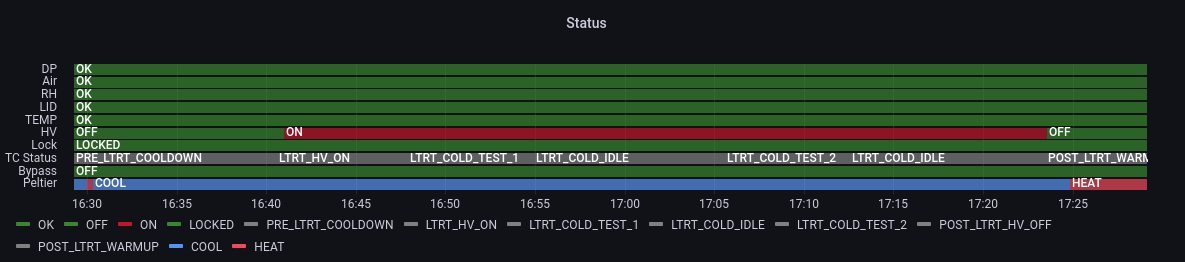
\includegraphics[width=14cm,height=11cm,keepaspectratio]{Figures/results/test_period.png}
    \caption{A record of two consecutive LTRT tests in the Influx database, showing the pre-tests, the LTRT test, and the waiting (IDLE) period between each test.}
    \label{fig:LTRTinflux}
\end{figure}

The first test was performed at $0 \si{\celsius}$ with $2$ iteration of LTRT and an interval of $10$ minutes between the two cold LTRTs. The timetable related to this test is shown in Fig\ref{fig:LTRTinflux}. The results of the ABCstar full test are shown in Fiq.\ref{fig:LTRT_result_1} and Fiq.\ref{fig:LTRT_result_2} showing the result of the two attempts of the performed test. (and Fiq.\ref{fig:LTRT_result_1_large} and Fiq.\ref{fig:LTRT_result_2_large} for higher resolution)

\begin{figure}[h]
    \begin{subfigure}[b]{0.45\textwidth}
        \centering
        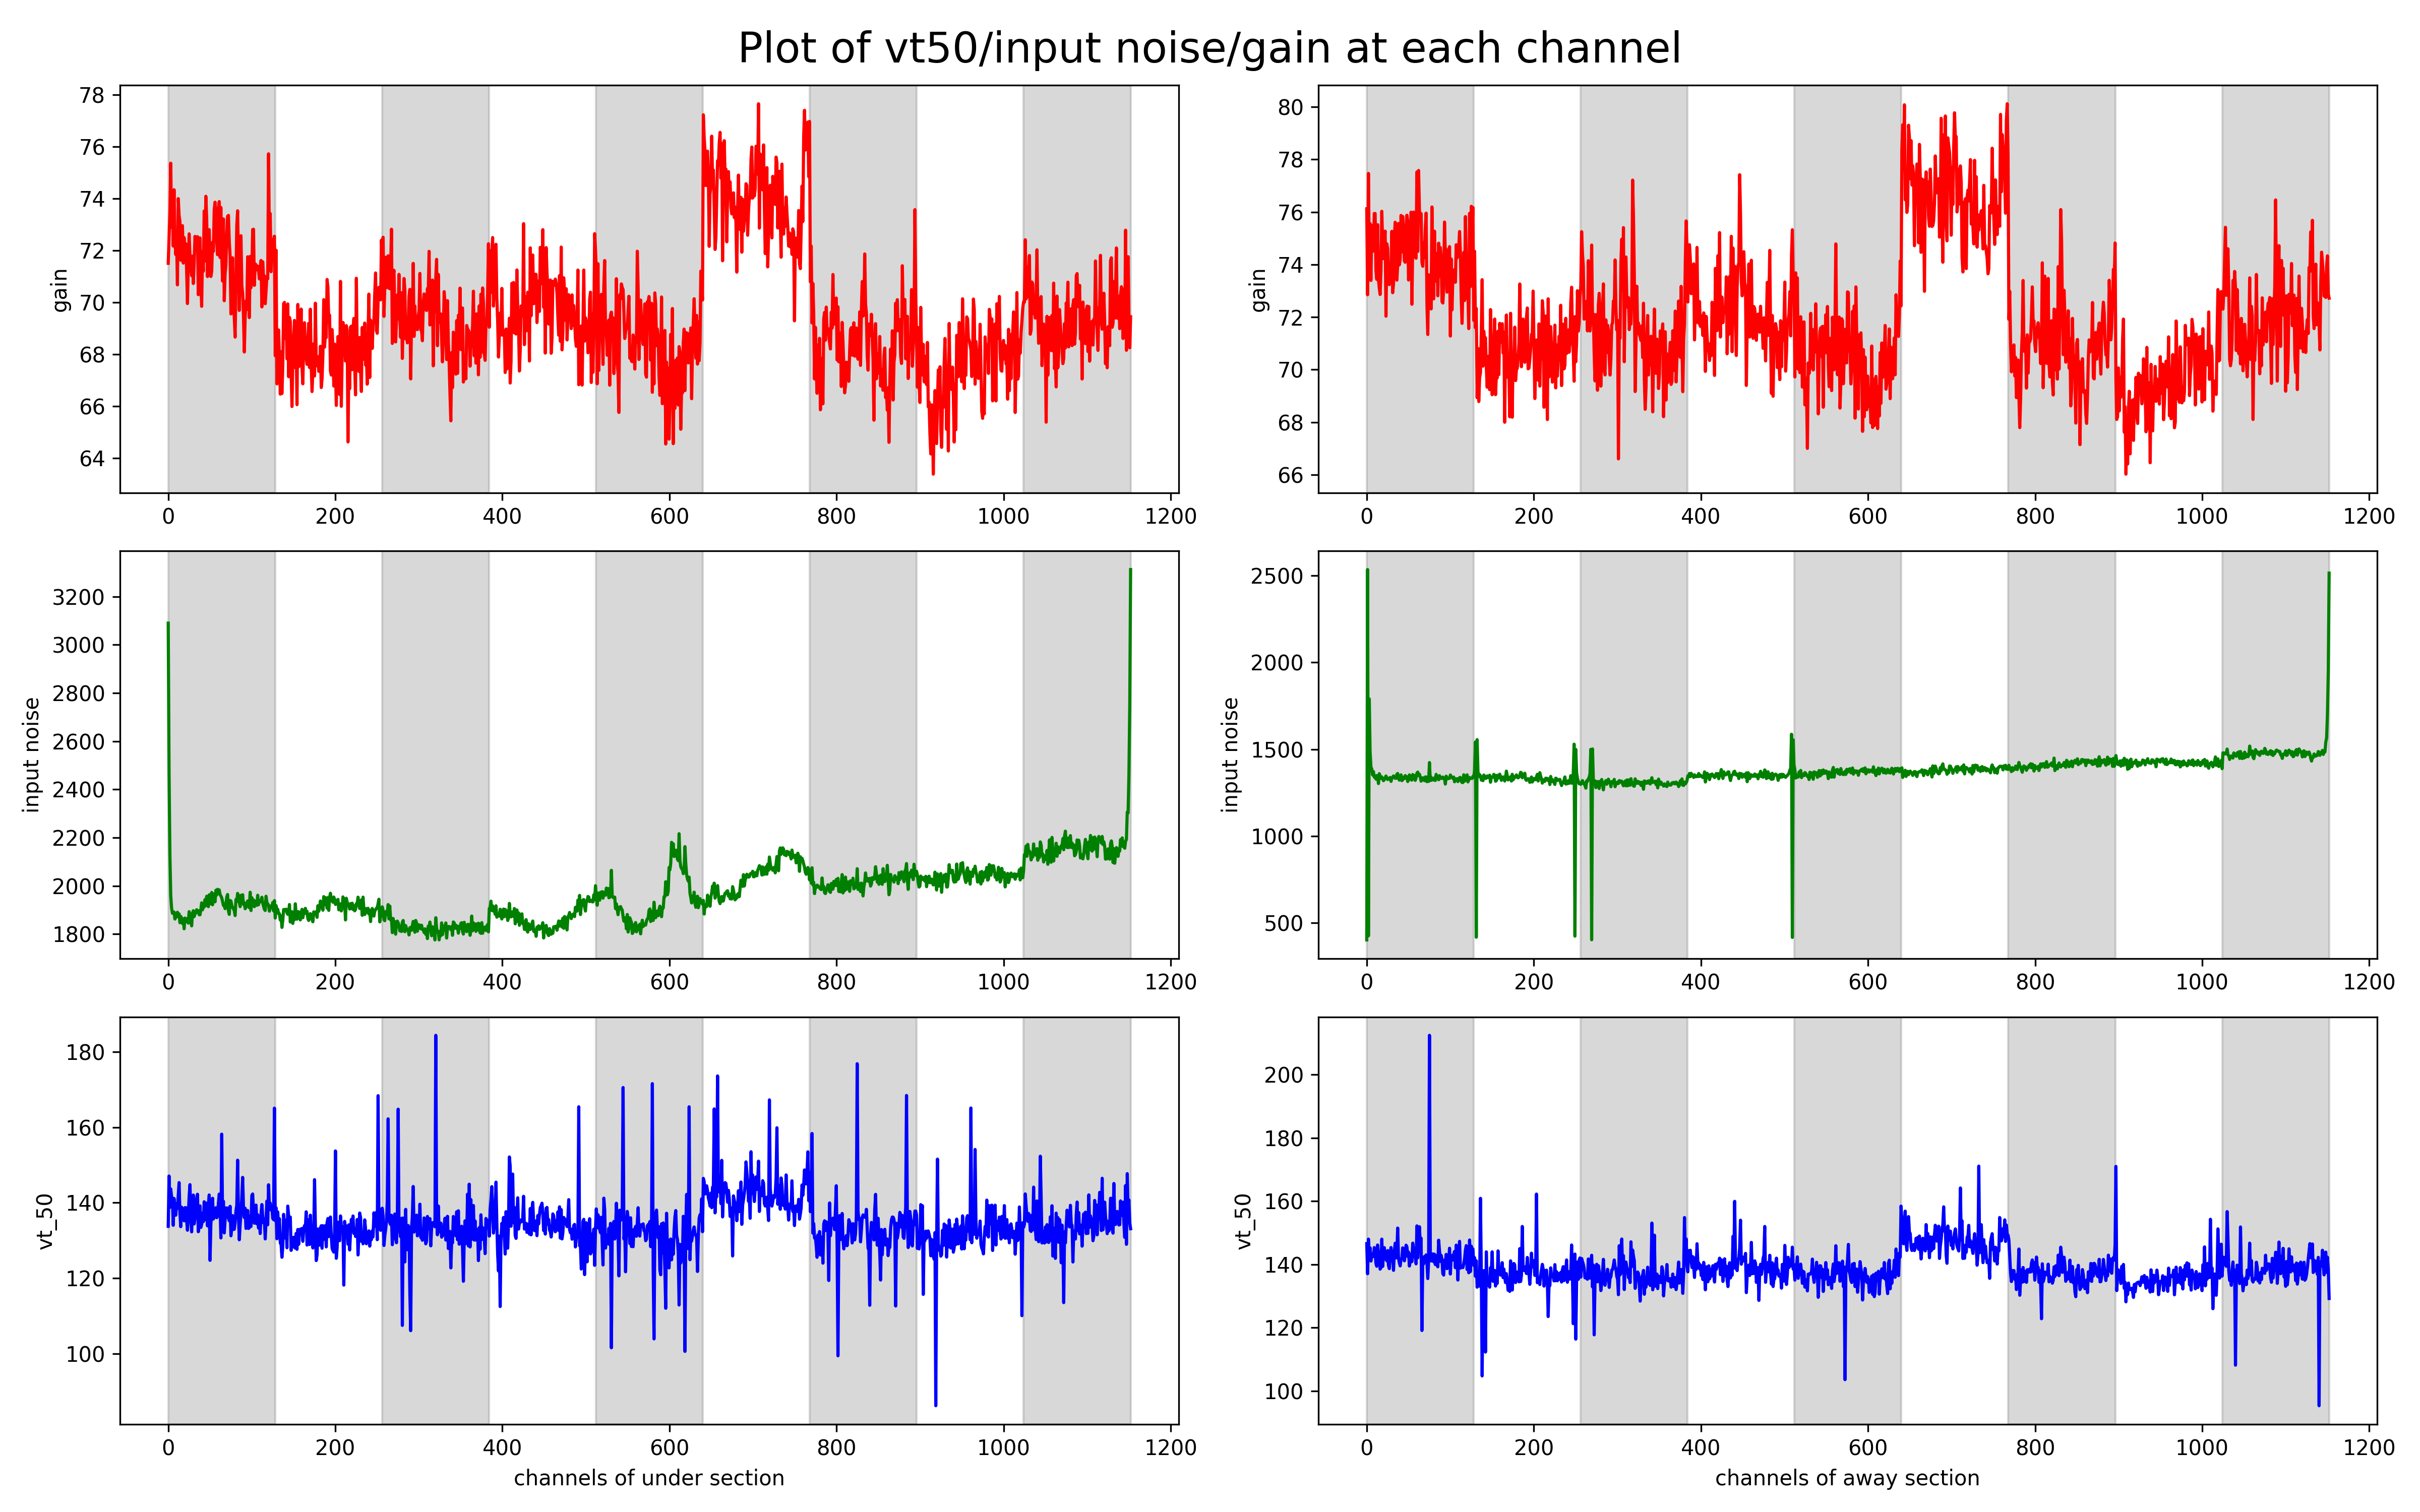
\includegraphics[width=7cm,height=10cm,keepaspectratio]{Figures/results/LTRT_1_plot.png}
        \caption{}
        \label{fig:LTRT_result_1}
    \end{subfigure}
    ~
    \begin{subfigure}[b]{0.45\textwidth}
        \centering
        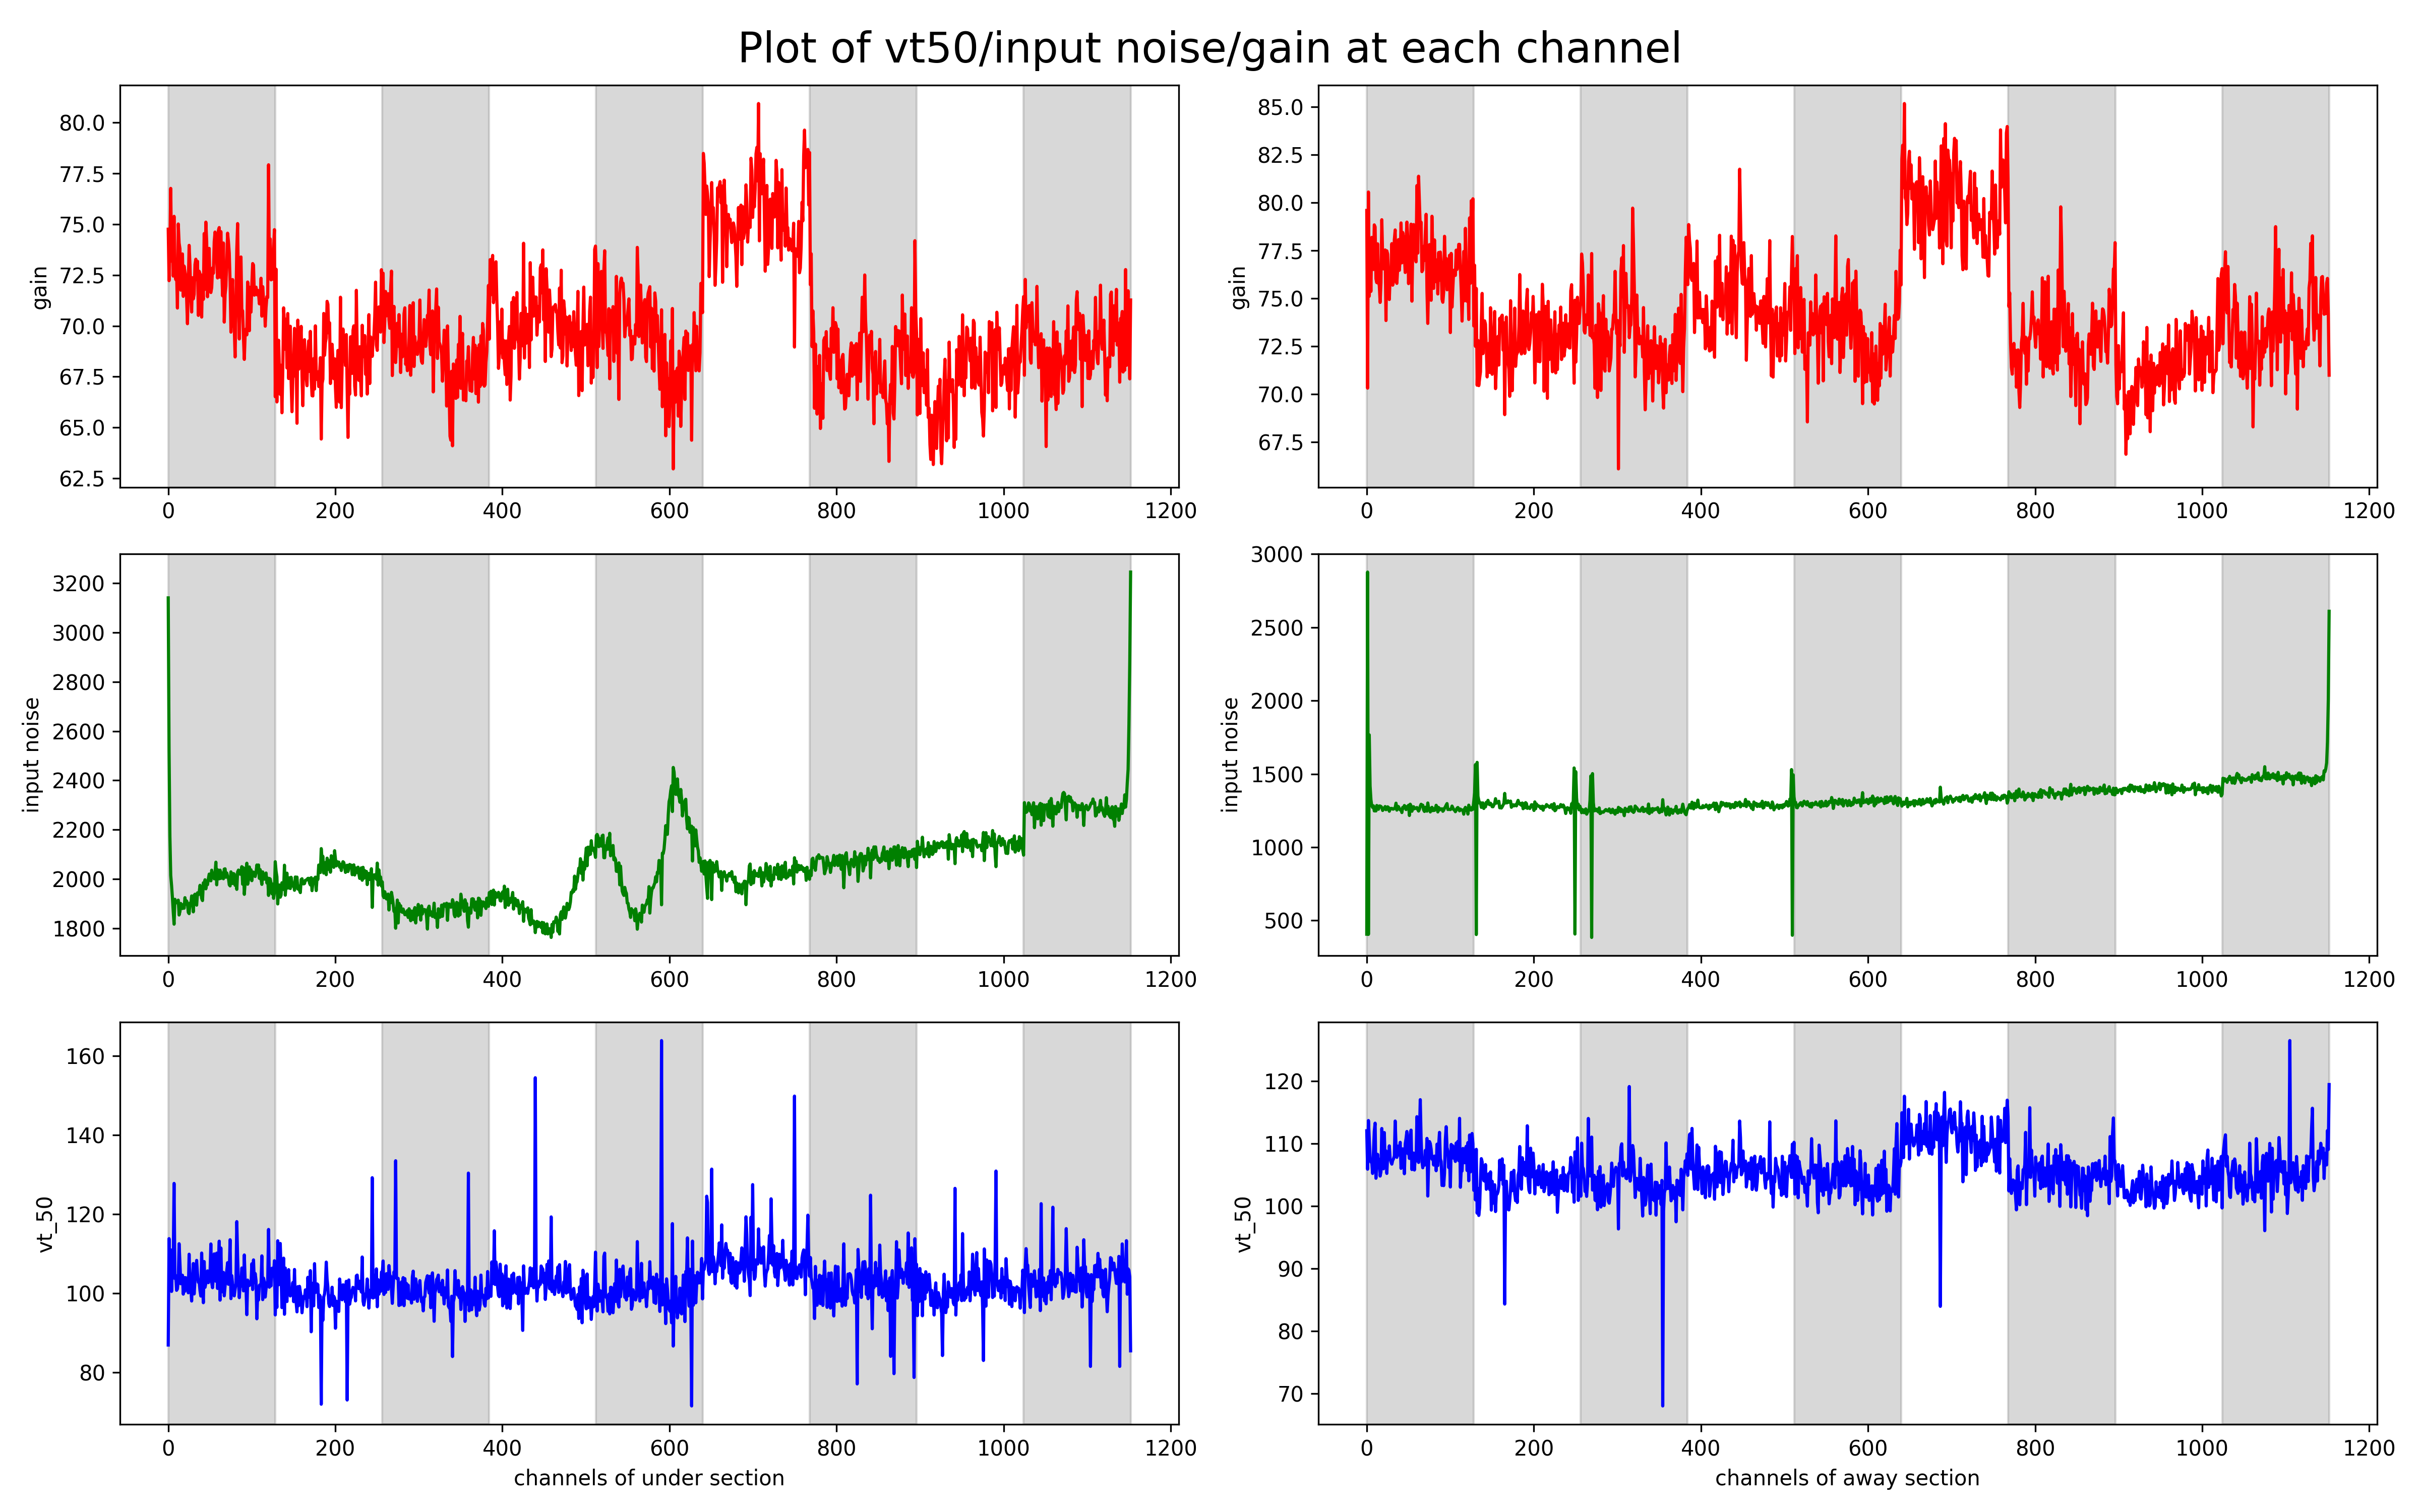
\includegraphics[width=7cm,height=10cm,keepaspectratio]{Figures/results/LTRT_2_plot.png}
        \caption{}
        \label{fig:LTRT_result_2}
    \end{subfigure}
    \caption{Plots of $3$ performed electrical test by ABCstar full test during the a) "LTRT COLD TEST 1" stage, and b) "LTRT COLD TEST 2" stage, showing the results of VT$50$, input noise, and gain for two hybrids (under and above) of a Pre Production A (PPA) R5 module.}
    
\end{figure}

Each point in the plots above shows the value of a single channel, and each highlighted area divides the data from each ABCstar readout (for this case $9$ readout per hybrid).\\

The environmental data related to both "LTRT COLD TEST 1" and "LTRT COLD TEST 2" and the "IDLE" period in between the two tests is shown in Fig.\ref{fig:env_1}(and Fiq.\ref{fig:env_1_large} for higher resolution)

\begin{figure}[h]
    \centering
    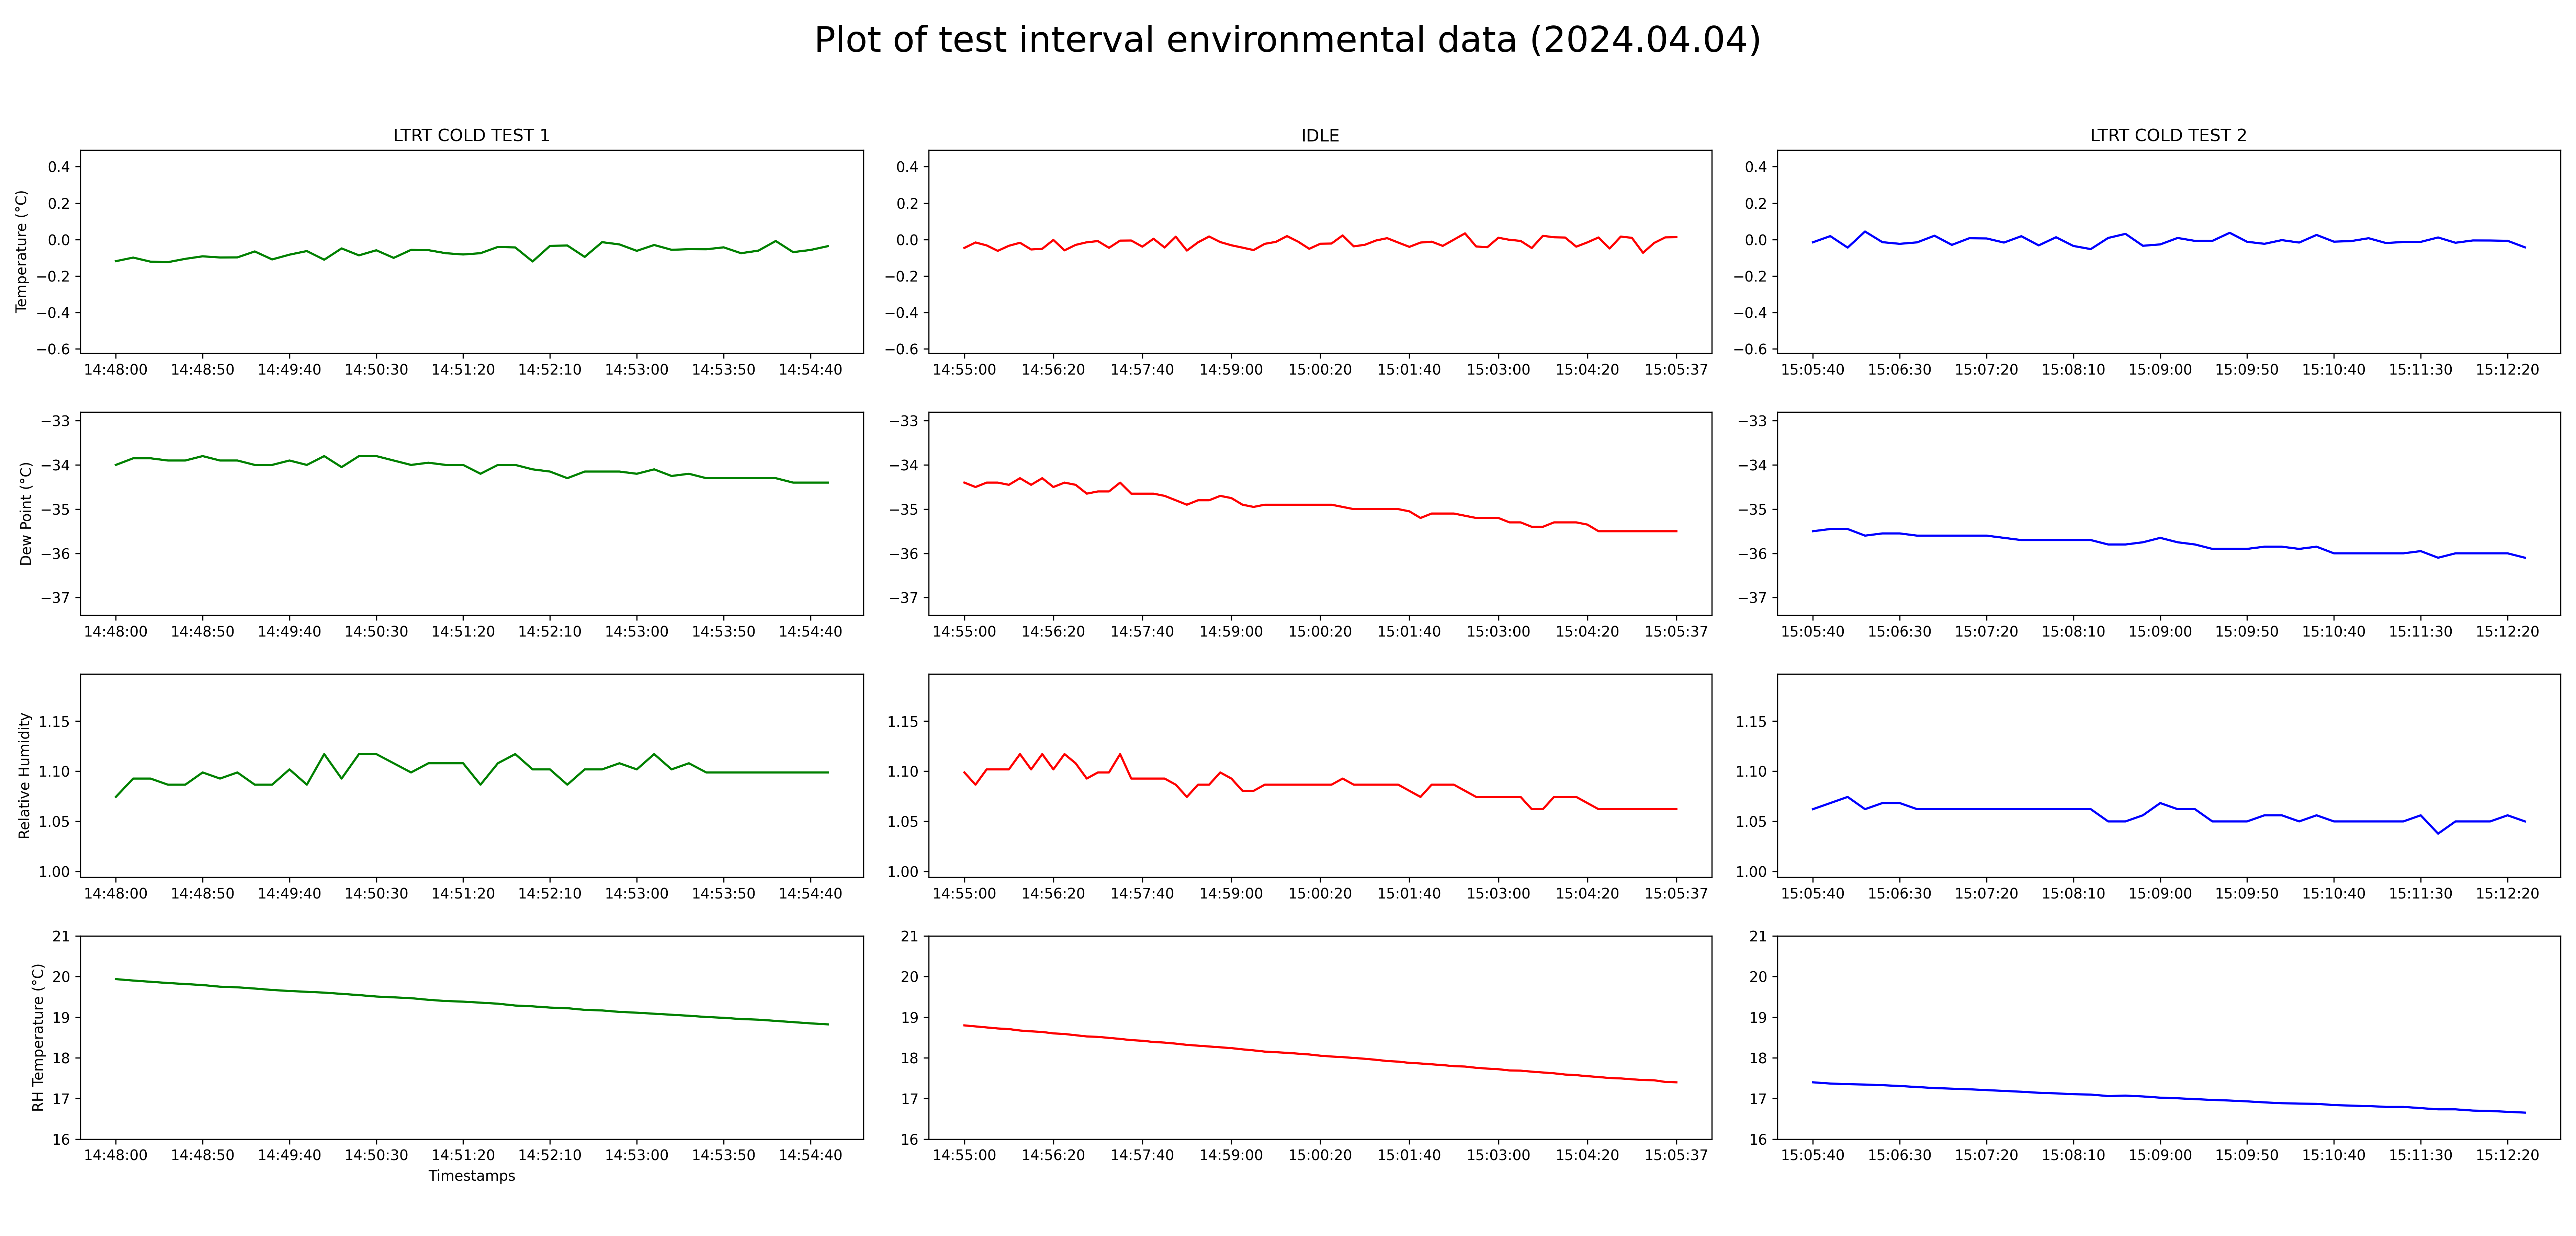
\includegraphics[width=12cm,height=10cm,keepaspectratio]{Figures/results/env_plot_20240404.png}
    \caption{Plots environmental data during the time span of the LTRT test shown in Fig.\ref{fig:LTRT_result_1} and Fig.\ref{fig:LTRT_result_2} showing the data for Temperature, Dew point, Relative humidity, and Relative humidity temperature.}
    \label{fig:env_1}
\end{figure}

The AMAC electrical data related to this test is shown in Fig.\ref{fig:amac_1}(and Fiq.\ref{fig:amac_1_large} for higher resolution)

\begin{figure}[h]
    \begin{subfigure}[b]{1\textwidth}
        \centering
        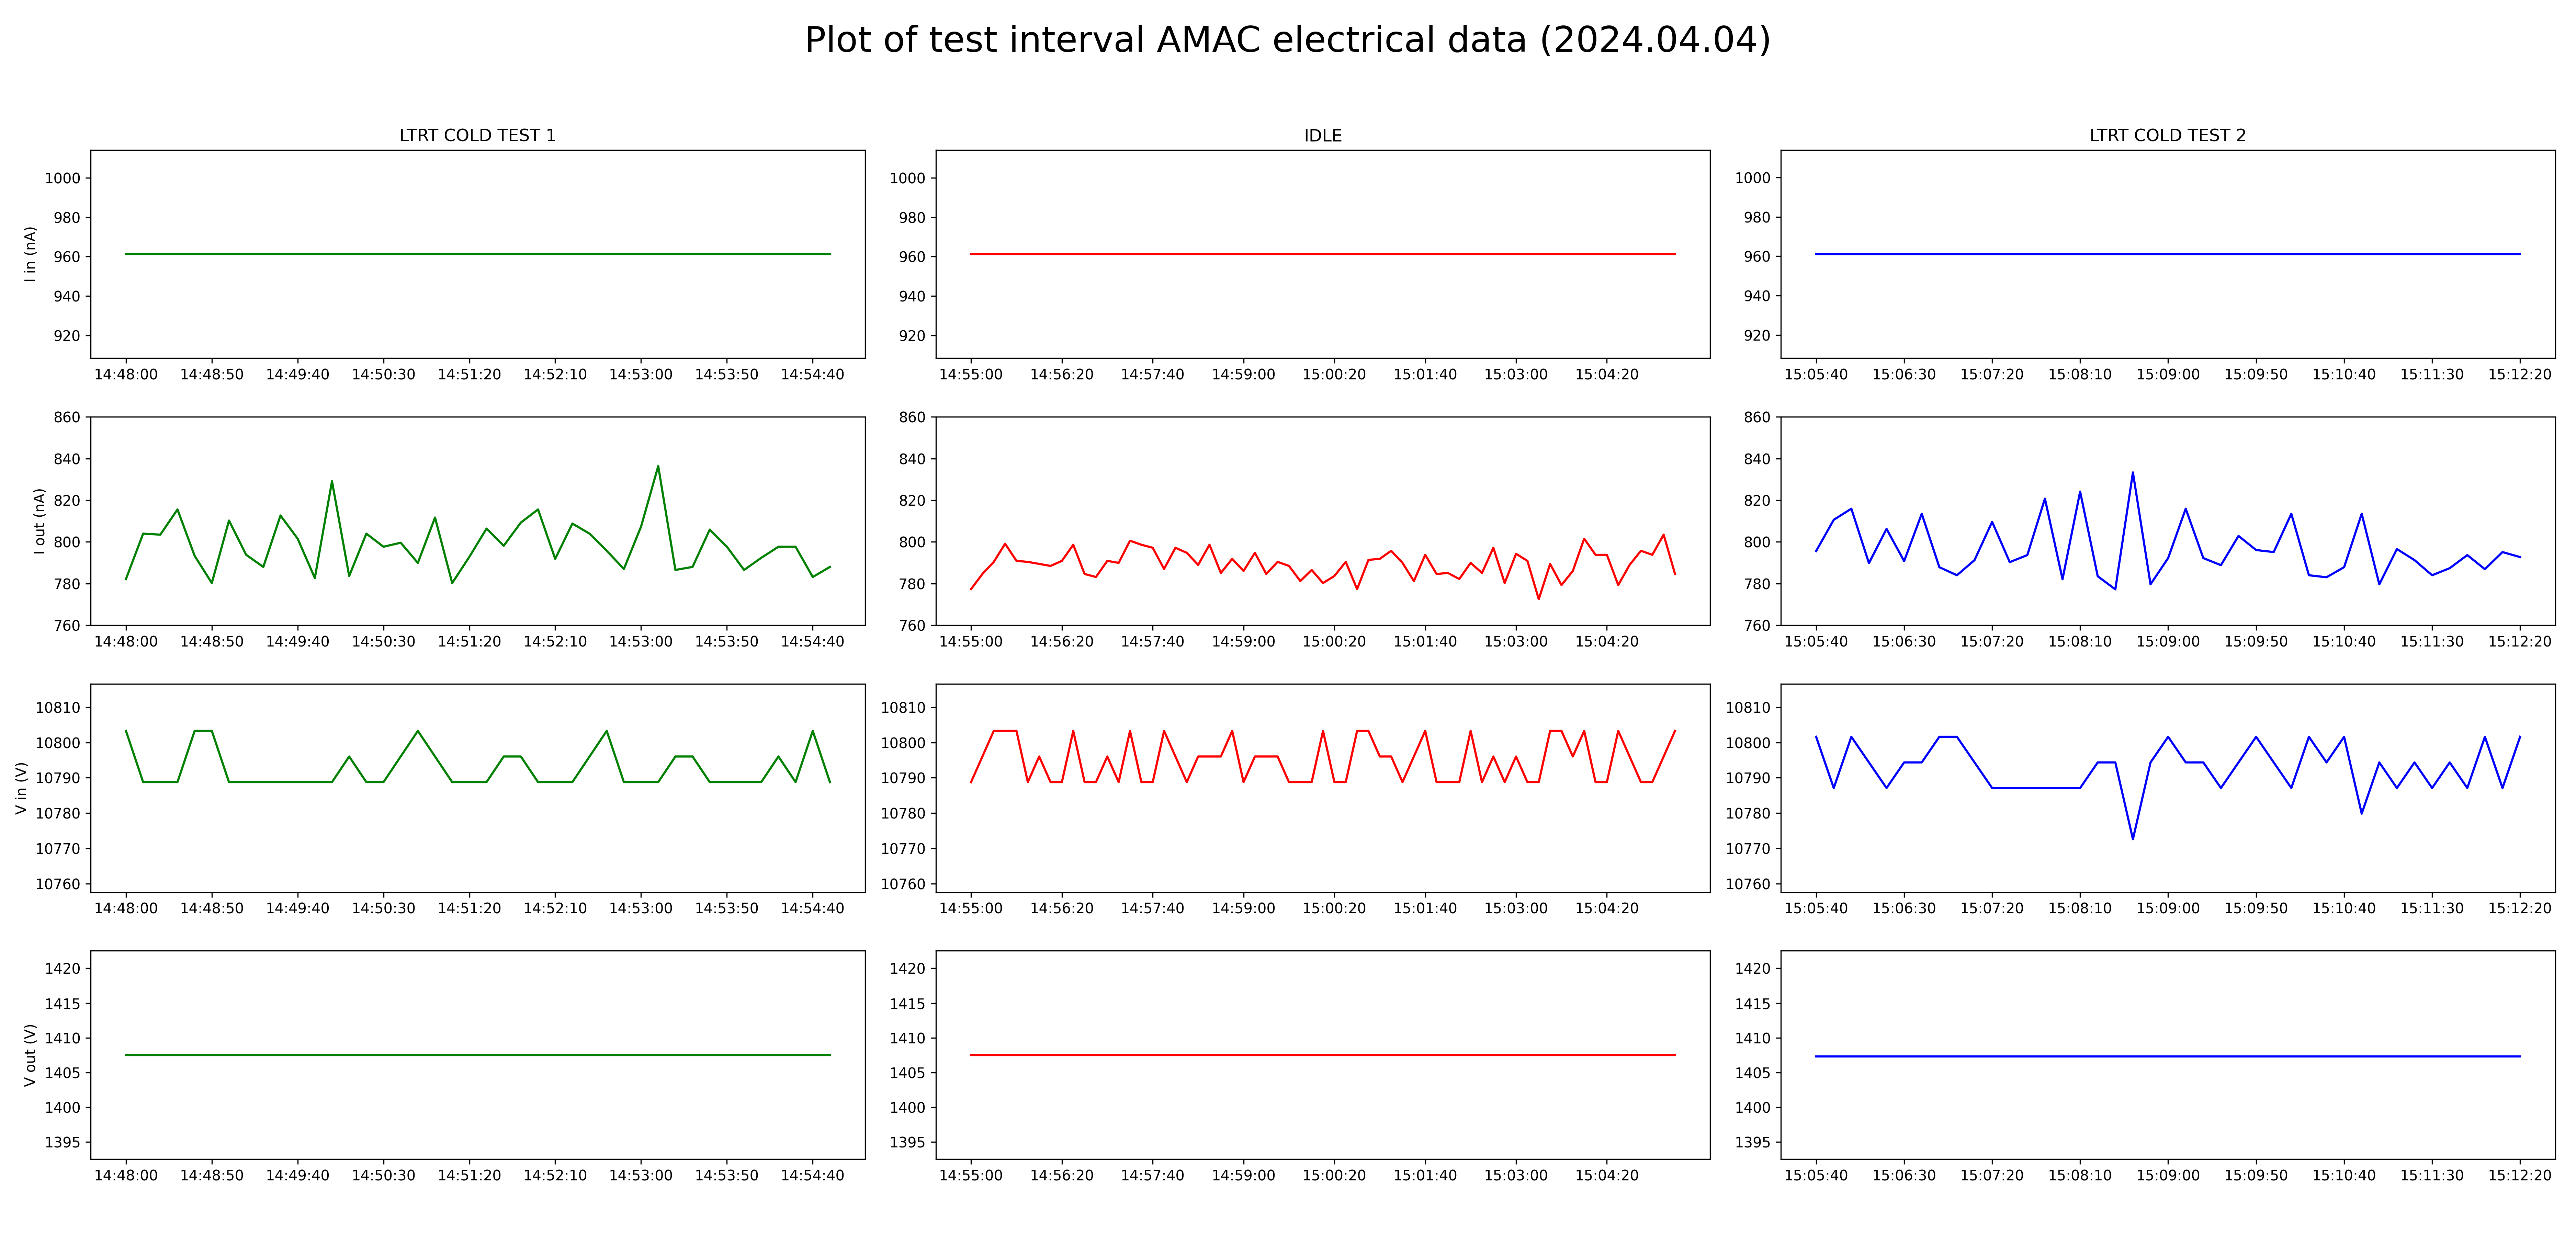
\includegraphics[width=12cm,height=10cm,keepaspectratio]{Figures/results/amac_el_plot_20240404_.png}
        \caption{}
        \label{fig:amac_el}
    \end{subfigure}
    ~
    \begin{subfigure}[b]{1\textwidth}
        \centering
        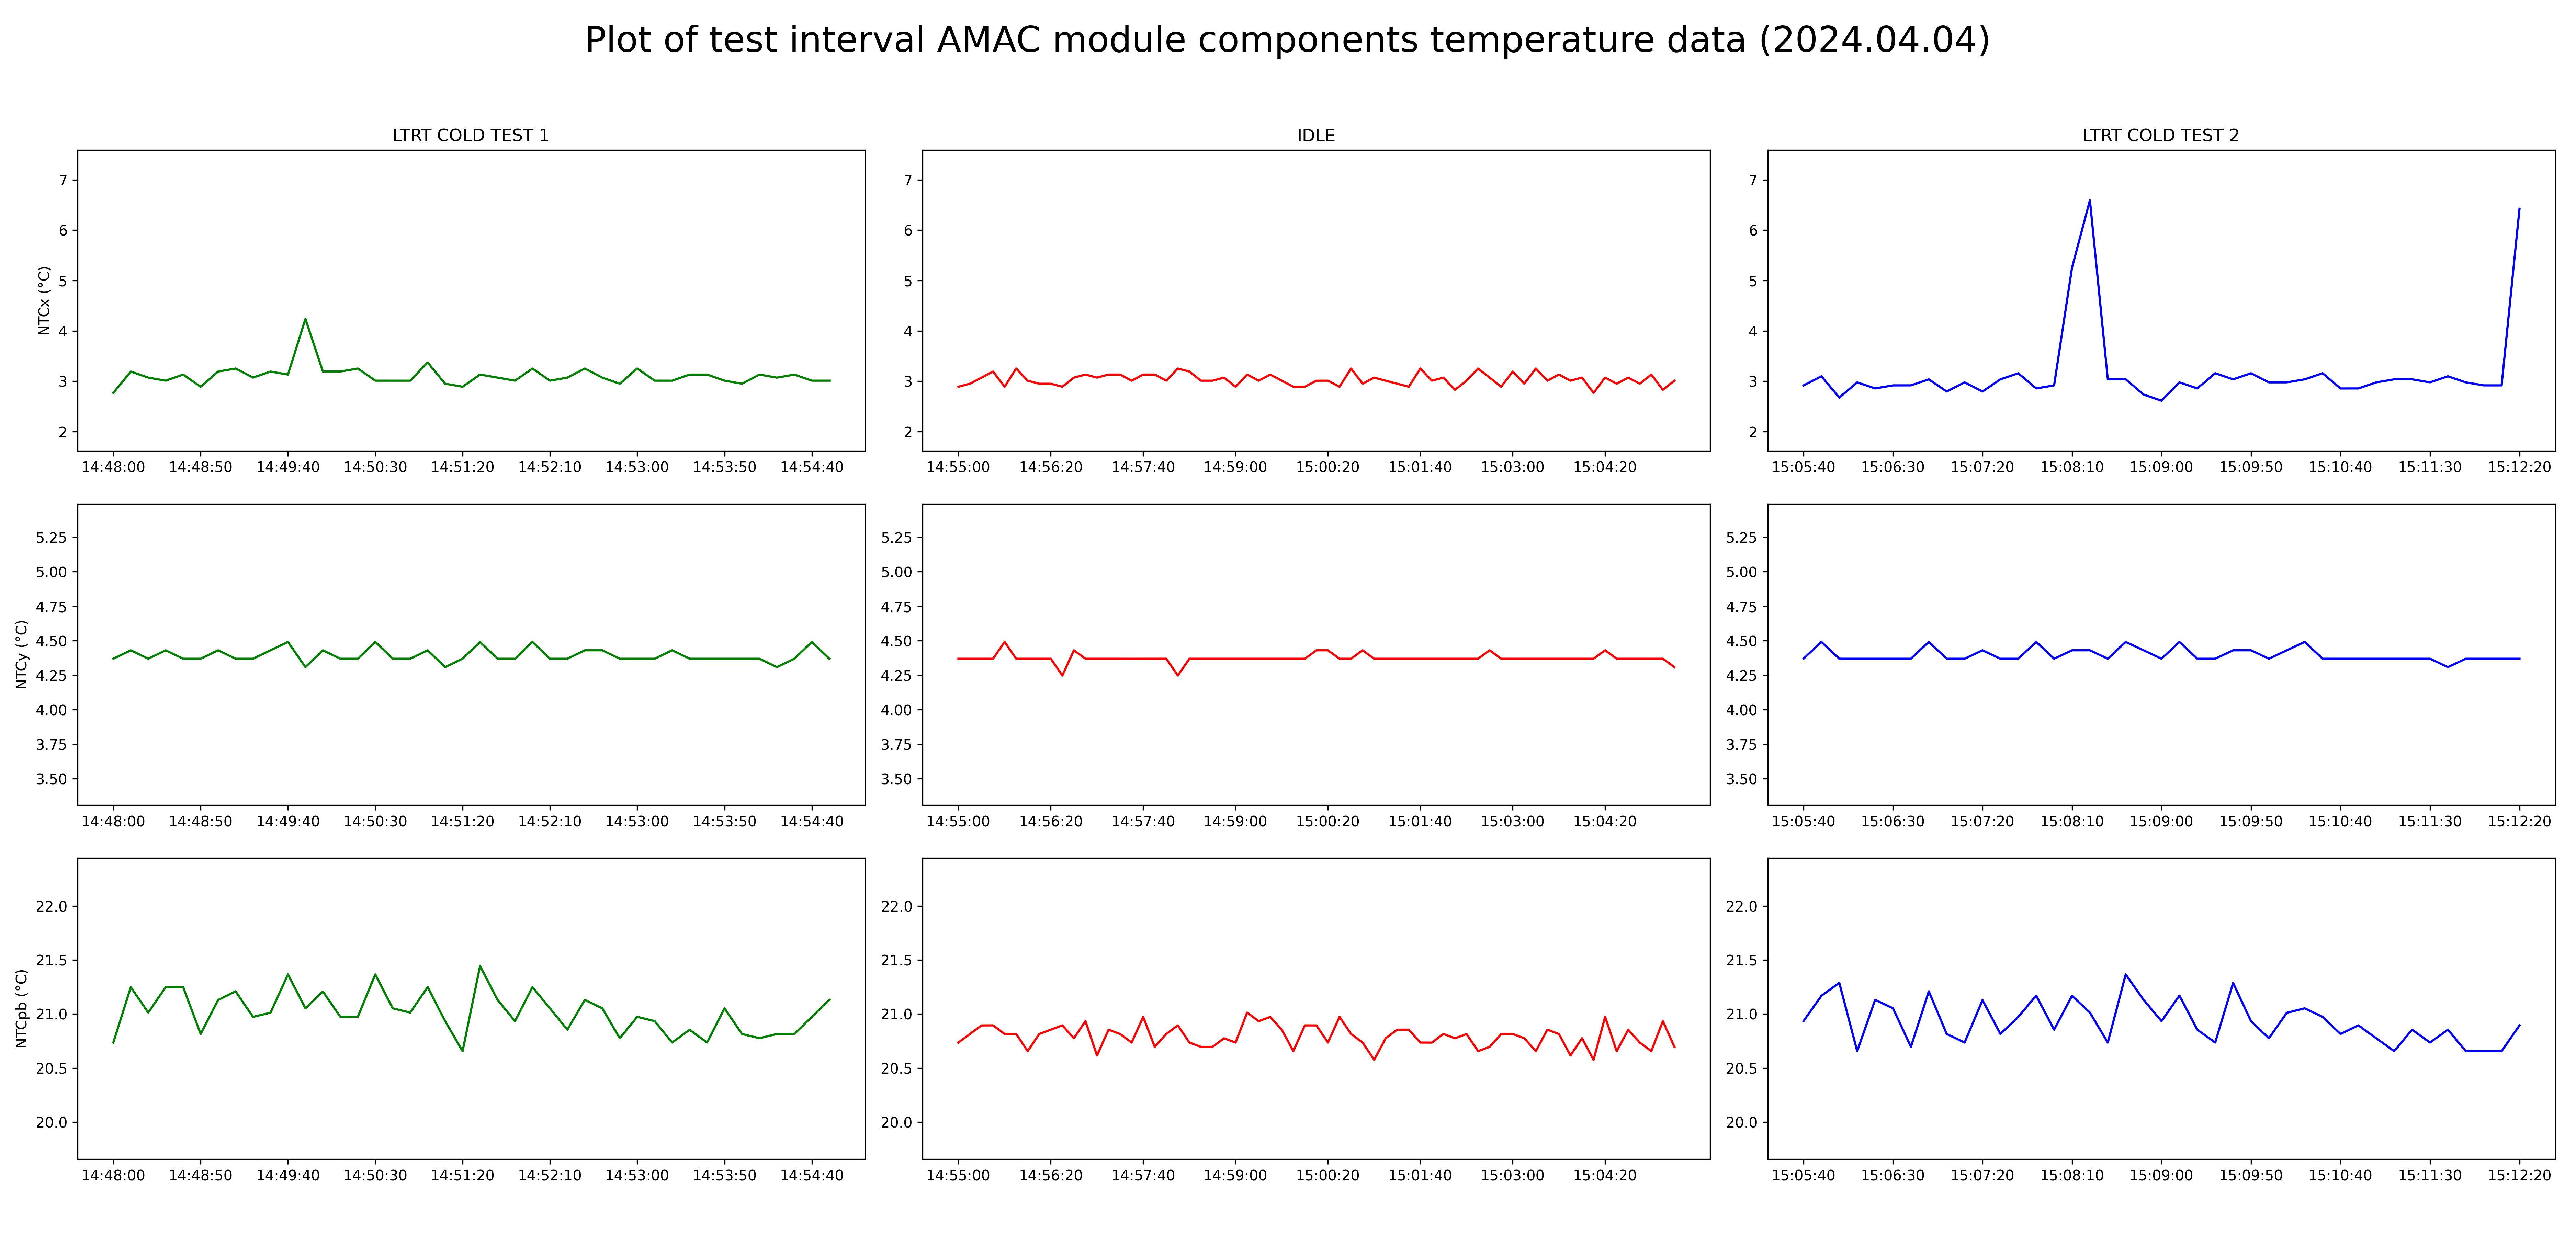
\includegraphics[width=12cm,height=10cm,keepaspectratio]{Figures/results/amac_temp_plot_20240404_.png}
        \caption{}
        \label{fig:amac_temp}
    \end{subfigure}
    \caption{Plots of a) AMAC electrical data showing the DC/DC input/output current (Iin/Iout), and input/output voltage of the DC/DC converter, and b) AMAC module components temperature showing the temperature on each of the hybrids (NTCx/NTCy) and powerboard (NTCpb), during the time span of the LTRT tests shown in Fig.\ref{fig:LTRT_result_1} and Fig.\ref{fig:LTRT_result_2}.}
    
\end{figure}

While the time taken for each test varies depending on the module, configuration, and settings, by aligning the ordered tests with the environmental and electrical data, we can have a general overview of the test conditions. \\
By checking the environmental plots we can determine that the temperature on the chuck on which the module was installed, was perfectly constant during the LTRT COLD TESTs and the IDLE period and was maintained at $0\si{\celsius}$. The dew point, however, is decreasing. Since the dew point is directly proportional to relative humidity and the air temperature, we can see that this change is a result of the decrease in relative humidity and the air temperature (RH Temp.) during the full test.\\

For the electrical results from the AMAC, we can see that we get two sets of data related to the DC/DC converter: input current and voltage, and output current and voltage. As shown in Fig.\ref{fig:amac_el}, the input current is at the stable level of $960\si{\nano\ampere}$, but the DC/DC converter is trying to regulate the current and stepping it down (Bucked) to sent the current to the components. On the other hand, the Votage is stepping up (Boosted) during the tests, and set on a stable level of $1407 \si{\volt}$.\textbf{WHY???}\\

The Temperature data from AMAC, as shown in Fig.\ref{fig:amac_temp} is showing the temperature on each hybrids (NTCx and NTCy \textbf{Which one is which?}) and the power board (NTCpb). Altough the figure shows fluctuations in the temperature during the tests, but aside from the two spikes on NTCx during the LTRT COLD TEST 2, it reflects a fairly good stability. However, the spikes on the temperature of NTCx could be the result of ...???

